\chapter{GATESIM METHODOLOGIES}
\label{chap:methodologies.tex}

Different methodologies could be adopted for netlist simulation and verification. First step would be to obtain the test vector stimulus that needs to be applied onto the netlist. One widely used method is to reuse the RTL testbench around the netlist. Another variant of this method could be to replace only a portion of circuit with netlist in the existing RTL verification environment.

Another method could be to capture test vectors from RTL simulation followed by applying it on corresponding netlist simulations. In such a method, comparison could be done between RTL behaviour (stored as captured test vectors) with that of netlist simulation.  In AMD, gatesim verification is accomplished by one such methodology. Over the years, two different methodologies were adopted for test vector capture and stimulus application. These are now called as {\it Early Dual-Sim methodology} and {\it Co-sim based Gatesim methodology}. Due to its many shortcomings, the early dual sim methodology was discontinued over Co-sim based Gatesim methodology. Co-sim based Gatesim is the current de-facto methodology for gate level simulations.


\section{EARLY DUAL-SIM METHODOLOGY}
Early method for gate level simulation was a dual-sim or simulation-after-simulation method. In this methodology RTL simulation was done initially with test bench components. The test vectors for gatesims were generated during this RTL simulation using ``\$display'' or VCD (value change dump). During netlist simulation, these test vectors were used as stimulus and comparison was done with the RTL output vectors. ~\figurename{~\ref{fig:early.ps}} shows the simulation flow. % Meera : 1. Figure x, 2. Have some good diagrams
%Naren: need this para re-write with references to figure

%\figurename{} 
\begin{figure}[h]
\centering
\includegraphics[width=4in, height=3.5in]{./figures/early.ps}
\caption{Early Dual-Sim Flow}
\label{fig:early.ps}
\end{figure}

This dual-sim method was widely used across industry due to its many advantages. The main advantage being best simulation performance with least compute requirements. However the earlier implementation of this method had multiple shortcomings which became more prevalent with increasing design complexity.

\paragraph{Shortcomings:}The main issue with earlier implementation of dual sim methodology was the huge disk space requirement. Vector files were text files which had cycle based stimulus information. These files were large and simulation performance was also affected by disk input/output accesses. Another shortcoming of this methodology was, when stimulus is converted to cycle based information sampling errors were introduced. At times, these sampling errors were themselves causing simulation mismatches when compared to RTL simulations.

 
 With increasing design complexity, the disk-space requirements became too high that the method could no longer be sustained and a new co-simulation based methodology was adopted instead.





\section{CO-SIM BASED GATESIM METHODOLOGY}
 Cosim-based methodology was conceived to solve some problems that existed with earlier dual-sim approach. To its advantage, the new method enabled ease of debug while maintaining consistent input vectors (devoid of sampling errors). It also made results comparision and debug easier. ~\figurename{~\ref{fig:cosim.ps}} shows how stimulus is applied to netlist and comparison of output is done in cosim method. %FIXME: Check last line
 
\begin{figure}[h!]
\centering
\includegraphics[width=4in, height=3.5in]{./figures/cosim.ps}
\caption{Co-sim Based Gatesim}
\label{fig:cosim.ps}
\end{figure}


 In Cosim methodology, a single combined simulation consisting of the netlist with behavioral RTL and stimulus components is made. In this simulation, behavioral RTL and gate models are run in lock-step with their inputs tied and the comparison of the behavioral RTL and gate outputs is done ``on the fly''. ~\figurename{~\ref{fig:cosim_flow.ps}} shows cosim flow.




%\figurename{} 
\begin{figure}[h]
\centering
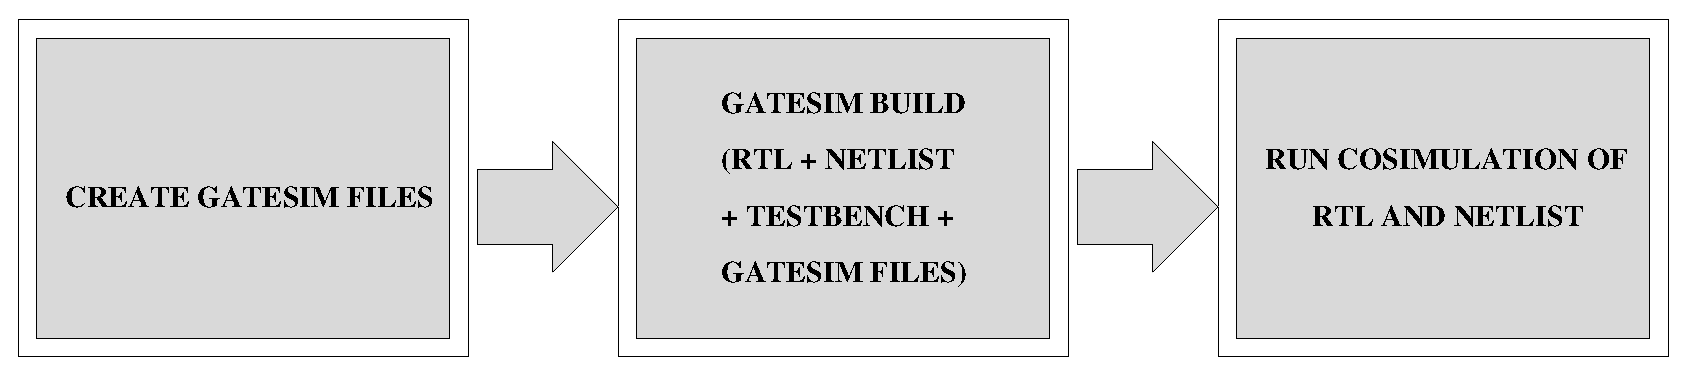
\includegraphics[width=4in, height=1.5in]{./figures/cosim_flow.ps}
\caption{Co-sim Based Gatesim Flow}
\label{fig:cosim_flow.ps}
\end{figure}

Major steps involved in this flow are:

\begin{enumerate}
	\item \emph{\bf Getting gatesim files}

	Input to gatesims are obtained from LEC flow. The list includes the netlist file, files holding information regarding IO/Register mapping, gate defines, compare enables and testbench force files. These inputs from LEC stage are processed by a set of scripts for developing intermediate files which are needed by cosim build infrastructure. These files are exclusively required for netlist simulations and described below
	\begin{itemize}
		\item[gatesim.v] instantiates top level netlist and ties its inputs with the behavioral RTL.
		\item[compare.v] contains comparators those compare the outputs and register mappings, for each cycle of simulation.
		\item[forces.v] contains all the force/release/assign commands for the gates corresponding to RTL force/release/assign statements. Forces are required in the design to shorten reset, initialize training parameters, initialize fuses among other things.
	\end{itemize}

	\item \emph{\bf Getting gatesim build} 

	Next stage is to enable a build structure supporting the co simulation of RTL and Netlist. The build includes:
	\begin{itemize}
		\item[-]Netlist to be verified
		\item[-]Complete RTL of SoC
		\item[-]Test bench components in its entirety
		\item[-]Gatesim files
	\end{itemize}

	\item \emph{\bf Run cosimulation of RTL and netlist}

	Running co-simulation is very similar to running RTL simulation. Output files include $<$testname$>$.out which contains the simulation transcript of the entire test and $<$testname$>$.fsdb (waveform dump file). The simulation transcript also contains gatesim errors called as ``miscompares''.
\end{enumerate}


As the netlist stimulus is obtained from a live RTL instead from stored vectors, cosim based gatesim overcame the biggest limitation associated with dual-sim. Over time, some good set of scripts aiding testbench generation, force generation were standardized. This method became the standard method for gatesims, close to a decade.

\subsection {LIMITATIONS OF CO-SIM METHODOLOGY}

Co-sim based Gatesim overcame all known limitations associated with early methodology. As design complexity grew, it brought in new set of unforeseen limitations. Of those, the important ones are already discussed in Section~\ref{intro:sec:ifg}.

In order to better understand these limitations certain experimental analysis were done. Experiments showed that the simulation performance of gatesim was affected sometimes as low as $10\%$ with respect to its counterpart RTL simulations. This indicates that:

\begin{itemize}
	\item[-]RTL Simulations contribute major to simulation performance than netlist.
	\item[-]Simulator spends more time in simulating RTL and verification components than netlist.
\end{itemize}

On further investigation it became clear that RTL simulation, which is simulated redundantly for the sole purpose of generating test vectors influences the simulation performance greatly. Such complex SOC design has multitude of Verification components in different programming languages including C, C++, SVTB, OVA, SVA and that these verification components take a big share of simulation cycles and have negative effect on simulation performance.

Evidently it was not an appropriate use of compute resources by having live RTL simulation every time, for the sole purpose of test vector generation. The analysis provides convincing evidence for us to attempt changes in existing cosim-based methodology.

